\documentclass{article} 
\usepackage{texthanglist}
\usepackage{changepage}
\usepackage{float}
\usepackage{grffile}
\usepackage{graphicx}
\usepackage{amssymb}
\usepackage{fontspec}
\usepackage{fancyhdr}
\usepackage{multicol}

\begin{document} 
\thispagestyle{empty} 
\font\spanxitemtranslationtranslationsexamplessensesensesentryletDatadicBody="Times New Roman" at 10pt
\font\xitemtranslationtranslationsexamplessensesensesentryletDatadicBody="Times New Roman" at 10pt
\font\translationtranslationsexamplessensesensesentryletDatadicBody="Times New Roman" at 10pt
\font\translationsexamplessensesensesentryletDatadicBody="Times New Roman" at 10pt
\font\spanexampleexamplessensesensesentryletDatadicBody="Times New Roman" at 10pt
\font\exampleexamplessensesensesentryletDatadicBody="Times New Roman" at 10pt
\font\examplessensesensesentryletDatadicBody="Times New Roman" at 10pt
\font\spanLexSensepublishStemGlossPubsensesensesentryletDatadicBody="Times New Roman" at 10pt
\font\LexSensepublishStemGlossPubsensesensesentryletDatadicBody="Times New Roman" at 10pt
\font\spandefinitionsensesensesentryletDatadicBody="Times New Roman" at 10pt
\font\definitionsensesensesentryletDatadicBody="Times New Roman" at 10pt
\font\xsensenumbersensesentryletDatadicBody="Times New Roman" at 10pt
\font\spanpartofspeechgrammaticalinfosensesensesentryletDatadicBody="Times New Roman" at 10pt
\font\partofspeechgrammaticalinfosensesensesentryletDatadicBody="Times New Roman" at 10pt
\font\grammaticalinfosensesensesentryletDatadicBody="Times New Roman" at 10pt
\font\sensesensesentryletDatadicBody="Times New Roman" at 10pt
\font\sensesentryletDatadicBody="Times New Roman" at 10pt
\font\spanpronunciationpronunciationsentryletDatadicBody="Times New Roman" at 10pt
\font\pronunciationpronunciationsentryletDatadicBody="Times New Roman" at 10pt
\font\pronunciationsentryletDatadicBody="Times New Roman" at 10pt
\font\headwordentryletDatadicBody="Times New Roman" at 10pt
\font\spanpictureLabelpictureCaptionpictureRightentryletDatadicBody="Times New Roman" at 10pt
\font\pictureLabelpictureCaptionpictureRightentryletDatadicBody="Times New Roman" at 10pt
\font\CmPicturepublishStemPileThumbnailPubpictureCaptionpictureRightentryletDatadicBody="Times New Roman" at 10pt
\font\pictureCaptionpictureRightentryletDatadicBody="Times New Roman" at 10pt
\font\picturepictureRightentryletDatadicBody="Times New Roman" at 10pt
\font\pictureRightentryletDatadicBody="Times New Roman" at 10pt
\font\entryletDatadicBody="Times New Roman" at 10pt
\font\letDatadicBody="Times New Roman" at 12pt
\font\letterletHeaddicBody="Gautami/B" at 24pt
\font\letHeaddicBody="Times New Roman" at 12pt
\begin{center}
\topskip 18pt{\letterletHeaddicBody{అ}}
 \label{first_pageఅ} \end{center}
\begin{adjustwidth}{1pt}{0pt}{2pt}{9pt}\begin{hanglist}[36pt] \item 
\begin{wrapfigure}
\begin{center}
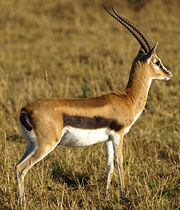
\includegraphics[angle=0,width=36mm,height=36mm]{c.jpg} 
\caption{}
\end{center}
\end{wrapfigure}


\spanpictureLabelpictureCaptionpictureRightentryletDatadicBody{rice with tumeric}

\leftmargin 36pt{\markboth{అక్సెదంగ్}{అక్సెదంగ్}\headwordentryletDatadicBody{అక్సెదంగ్}}\spanpronunciationpronunciationsentryletDatadicBody{aksedaṅg}\spanpartofspeechgrammaticalinfosensesensesentryletDatadicBody{n}\xsensenumbersensesentryletDatadicBody{1}\spandefinitionsensesensesentryletDatadicBody{rice with vermilion}\spanLexSensepublishStemGlossPubsensesensesentryletDatadicBody{rice with vermilion}\xsensenumbersensesentryletDatadicBody{2}\spandefinitionsensesensesentryletDatadicBody{rice mixed with vermilion thrown at a wedding, or on cattle (e.g. during 'laxmi pooja') in order to bless.}\spanLexSensepublishStemGlossPubsensesensesentryletDatadicBody{rice with turmeric used to bless}\spanexampleexamplessensesensesentryletDatadicBody{గొవుర్ దన్ గోటమ్నె నొవ్రి నొవ్రనగ సమ్దిర్ అక్సెదాంగ్ వాటంతెర్.}\spanxitemtranslationtranslationsexamplessensesensesentryletDatadicBody{At the wedding place, everyone throws rice on the bride andgroom.}\spanxitemtranslationtranslationsexamplessensesensesentryletDatadicBody{$\sharp$పెండ్లి పందిరిలో పడుసు, వరులకు పసుపు బియ్యం వేస్తారు.}\end{hanglist} \end{adjustwidth} 

\end{document}
